The Standard Model of particle physics, which describes three out of the four fundamental forces of nature, has been enormously successful at predicting and describing the particles we see in nature. Apart from the known fundamental particles, i.e.\ the quarks, leptons, gauge bosons, and the Higgs boson, many of the particles we encounter in nature are composite particles known as \emph{hadrons}. Similar to how an atom consists of protons, electrons, and neutrons, with the former two being bound together by the electromagnetic force, hadrons consist of quarks and gluons bound together by the strong nuclear force. The strong force is also responsible for binding protons and neutrons together in the nucleus of an atom.  While protons and electrons carry electric charge, quarks and gluons carry another type of charge known as \emph{color} charge (though quarks also carry electric charge).

While the electromagnetic force and its associated electric charge are described by the U(1) gauge theory of Quantum \emph{Electrodynamics} (QED), the strong force and its associated color charge are described by the SU(3) gauge theory of Quantum \emph{Chromodyamics} (QCD)~\cite{Fritzsch:1973pi}. One of the main reasons QED has been so useful for analytic calculations is because the coupling of the theory is small enough that most quantities can be calculated perturbatively. QCD, however, has a \emph{running coupling} which becomes large low energy scales, preventing the theory from being amenable to perturbative methods except for at high energies. A plot of the QCD coupling as a function of the energy scale is shown in Fig.~\ref{fig:alpha_s}. This phenomenon, known as \emph{asymptotic freedom} was shown independently by Gross and Wilczek~\cite{Gross:1973id} and by Politzer~\cite{Politzer:1973fx}, and is named as such because at high energies quarks are no longer bound together. While QCD is analytically tractable at high energies ($\sim m_Z$) and can be approached with Chiral Perturbation Theory, an effective low-energy theory of QCD, at low energies ($\sim m_\pi$), the intermediate range ($\sim 1$ GeV) is a region where analytic methods fail and non-perturbative methods are needed.

\begin{figure}
    \centering
    \hspace*{-0.1in}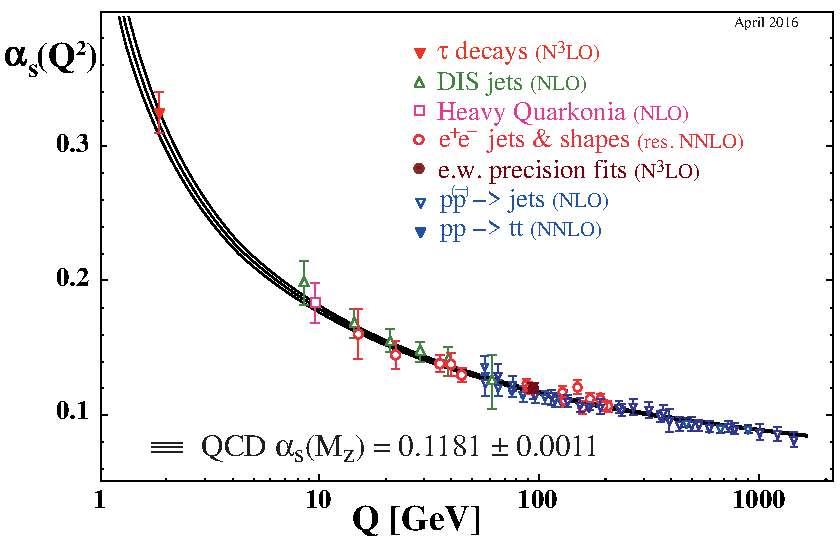
\includegraphics[width=0.8\textwidth]{figures/alpha_s.pdf}
    \caption[Plot of the QCD coupling $\alpha_s$ as a function of energy scale $Q$.]{Plot of the QCD coupling $\alpha_s$ as a function of energy scale $Q$. The respective degree of QCD perturbation theory used in the extraction of $\alpha_s$ is indicated in brackets. Figure taken from Ref.~\cite{PhysRevD.98.030001}.}\label{fig:alpha_s}
\end{figure}

The most successful non-perturbative method thus far for doing calculations in QCD is \emph{Lattice QCD}, which is an \emph{ab initio} method of simulating a discretized version of QCD on a spacetime lattice using Monte Carlo methods. The field of Lattice QCD began with Ken Wilson's famous 1974 paper~\cite{Wilson:1974sk} which showed how to quantize a gauge field theory on a discrete lattice in Euclidean spacetime while preserving exact gauge invariance.

Lattice QCD calculations are very computationally expensive, often requiring hundreds of millions of core hours to perform.~\cite{Fallica2018} In order to ease computational burdens, early calculations used coarse lattices, used very heavy pion masses (which ease the process of inverting very large Dirac matrices), and worked in the so-called ``quenched approximation'' wherein the effects of sea quarks are ignored. Additionally, many (even recent works) ignore the effects of disconnected diagrams in the evaluation of quark propagators, which also amounts to partially ignoring sea-quark effects. The need for an efficient method of performing lattice calculations of fully dynamical QCD neglecting no disconnected contributions has been recently satisfied by the \emph{Stochastic LapH method}~\cite{Morningstar:2011ka}, which is used in this work to study tetraquarks operators in the light scalar sector and the excited $\Sigma$ baryon spectrum. Both of these endeavors are difficult if not impossible to approach without a method such as the Stochastic LapH method, due to disconnected contributions that appear when working with multi-hadron operators that are important in the determination of the excited baryon spectrum and when working with tetraquark operators.

This work is organized as follows. In Chapter~\ref{ch:latticeqcd}, we outline the basic theory underpinning lattice QCD, including how QCD is formulated in discretized spacetime, the path integral approach to calculating observables, and some of the computational details of how our gauge field configurations are generated in such a path integral approach. In Chapter~\ref{ch:operators}, we delve into the details of how to construct quantum operators which create and annihilate the states we wish to study. In Chapter~\ref{ch:montecarlo}, we discuss how to calculate the two-point correlation functions used to extract the energy spectrum, and expound upon how the Stochastic LapH method is used to invert the large Dirac matrices involved in our calculations. In Chapter~\ref{ch:analysis}, we discuss our data analysis procedure which allows us to fit the correlator data we obtain to extract the finite-volume spectrum of QCD. In Chapter~\ref{ch:tetraquarks}, we present results on including tetraquark operators in the sectors containing the $\kappa$ and $a_0(980)$ mesons. In Chapter~\ref{ch:sigmas}, we present results on the excited $\Sigma$ baryon spectrum. Finally, we summarize our results in Chapter~\ref{ch:conclusions}.